% Options for packages loaded elsewhere
\PassOptionsToPackage{unicode}{hyperref}
\PassOptionsToPackage{hyphens}{url}
\PassOptionsToPackage{dvipsnames,svgnames,x11names}{xcolor}
%
\documentclass[
]{memoir}
\title{Data Science per psicologi}
\author{Corrado Caudek}
\date{2021-10-10}

\usepackage{amsmath,amssymb}
\usepackage{lmodern}
\usepackage{iftex}
\ifPDFTeX
  \usepackage[T1]{fontenc}
  \usepackage[utf8]{inputenc}
  \usepackage{textcomp} % provide euro and other symbols
\else % if luatex or xetex
  \usepackage{unicode-math}
  \defaultfontfeatures{Scale=MatchLowercase}
  \defaultfontfeatures[\rmfamily]{Ligatures=TeX,Scale=1}
  \setmonofont[]{Inconsolata}
\fi
% Use upquote if available, for straight quotes in verbatim environments
\IfFileExists{upquote.sty}{\usepackage{upquote}}{}
\IfFileExists{microtype.sty}{% use microtype if available
  \usepackage[]{microtype}
  \UseMicrotypeSet[protrusion]{basicmath} % disable protrusion for tt fonts
}{}
\makeatletter
\@ifundefined{KOMAClassName}{% if non-KOMA class
  \IfFileExists{parskip.sty}{%
    \usepackage{parskip}
  }{% else
    \setlength{\parindent}{0pt}
    \setlength{\parskip}{6pt plus 2pt minus 1pt}}
}{% if KOMA class
  \KOMAoptions{parskip=half}}
\makeatother
\usepackage{xcolor}
\IfFileExists{xurl.sty}{\usepackage{xurl}}{} % add URL line breaks if available
\IfFileExists{bookmark.sty}{\usepackage{bookmark}}{\usepackage{hyperref}}
\hypersetup{
  pdftitle={Data Science per psicologi},
  pdfauthor={Corrado Caudek},
  colorlinks=true,
  linkcolor={Maroon},
  filecolor={Maroon},
  citecolor={Blue},
  urlcolor={Blue},
  pdfcreator={LaTeX via pandoc}}
\urlstyle{same} % disable monospaced font for URLs
\usepackage{color}
\usepackage{fancyvrb}
\newcommand{\VerbBar}{|}
\newcommand{\VERB}{\Verb[commandchars=\\\{\}]}
\DefineVerbatimEnvironment{Highlighting}{Verbatim}{commandchars=\\\{\}}
% Add ',fontsize=\small' for more characters per line
\usepackage{framed}
\definecolor{shadecolor}{RGB}{248,248,248}
\newenvironment{Shaded}{\begin{snugshade}}{\end{snugshade}}
\newcommand{\AlertTok}[1]{\textcolor[rgb]{0.94,0.16,0.16}{#1}}
\newcommand{\AnnotationTok}[1]{\textcolor[rgb]{0.56,0.35,0.01}{\textbf{\textit{#1}}}}
\newcommand{\AttributeTok}[1]{\textcolor[rgb]{0.77,0.63,0.00}{#1}}
\newcommand{\BaseNTok}[1]{\textcolor[rgb]{0.00,0.00,0.81}{#1}}
\newcommand{\BuiltInTok}[1]{#1}
\newcommand{\CharTok}[1]{\textcolor[rgb]{0.31,0.60,0.02}{#1}}
\newcommand{\CommentTok}[1]{\textcolor[rgb]{0.56,0.35,0.01}{\textit{#1}}}
\newcommand{\CommentVarTok}[1]{\textcolor[rgb]{0.56,0.35,0.01}{\textbf{\textit{#1}}}}
\newcommand{\ConstantTok}[1]{\textcolor[rgb]{0.00,0.00,0.00}{#1}}
\newcommand{\ControlFlowTok}[1]{\textcolor[rgb]{0.13,0.29,0.53}{\textbf{#1}}}
\newcommand{\DataTypeTok}[1]{\textcolor[rgb]{0.13,0.29,0.53}{#1}}
\newcommand{\DecValTok}[1]{\textcolor[rgb]{0.00,0.00,0.81}{#1}}
\newcommand{\DocumentationTok}[1]{\textcolor[rgb]{0.56,0.35,0.01}{\textbf{\textit{#1}}}}
\newcommand{\ErrorTok}[1]{\textcolor[rgb]{0.64,0.00,0.00}{\textbf{#1}}}
\newcommand{\ExtensionTok}[1]{#1}
\newcommand{\FloatTok}[1]{\textcolor[rgb]{0.00,0.00,0.81}{#1}}
\newcommand{\FunctionTok}[1]{\textcolor[rgb]{0.00,0.00,0.00}{#1}}
\newcommand{\ImportTok}[1]{#1}
\newcommand{\InformationTok}[1]{\textcolor[rgb]{0.56,0.35,0.01}{\textbf{\textit{#1}}}}
\newcommand{\KeywordTok}[1]{\textcolor[rgb]{0.13,0.29,0.53}{\textbf{#1}}}
\newcommand{\NormalTok}[1]{#1}
\newcommand{\OperatorTok}[1]{\textcolor[rgb]{0.81,0.36,0.00}{\textbf{#1}}}
\newcommand{\OtherTok}[1]{\textcolor[rgb]{0.56,0.35,0.01}{#1}}
\newcommand{\PreprocessorTok}[1]{\textcolor[rgb]{0.56,0.35,0.01}{\textit{#1}}}
\newcommand{\RegionMarkerTok}[1]{#1}
\newcommand{\SpecialCharTok}[1]{\textcolor[rgb]{0.00,0.00,0.00}{#1}}
\newcommand{\SpecialStringTok}[1]{\textcolor[rgb]{0.31,0.60,0.02}{#1}}
\newcommand{\StringTok}[1]{\textcolor[rgb]{0.31,0.60,0.02}{#1}}
\newcommand{\VariableTok}[1]{\textcolor[rgb]{0.00,0.00,0.00}{#1}}
\newcommand{\VerbatimStringTok}[1]{\textcolor[rgb]{0.31,0.60,0.02}{#1}}
\newcommand{\WarningTok}[1]{\textcolor[rgb]{0.56,0.35,0.01}{\textbf{\textit{#1}}}}
\usepackage{longtable,booktabs,array}
\usepackage{calc} % for calculating minipage widths
% Correct order of tables after \paragraph or \subparagraph
\usepackage{etoolbox}
\makeatletter
\patchcmd\longtable{\par}{\if@noskipsec\mbox{}\fi\par}{}{}
\makeatother
% Allow footnotes in longtable head/foot
\IfFileExists{footnotehyper.sty}{\usepackage{footnotehyper}}{\usepackage{footnote}}
\makesavenoteenv{longtable}
\usepackage{graphicx}
\makeatletter
\def\maxwidth{\ifdim\Gin@nat@width>\linewidth\linewidth\else\Gin@nat@width\fi}
\def\maxheight{\ifdim\Gin@nat@height>\textheight\textheight\else\Gin@nat@height\fi}
\makeatother
% Scale images if necessary, so that they will not overflow the page
% margins by default, and it is still possible to overwrite the defaults
% using explicit options in \includegraphics[width, height, ...]{}
\setkeys{Gin}{width=\maxwidth,height=\maxheight,keepaspectratio}
% Set default figure placement to htbp
\makeatletter
\def\fps@figure{htbp}
\makeatother
\setlength{\emergencystretch}{3em} % prevent overfull lines
\providecommand{\tightlist}{%
  \setlength{\itemsep}{0pt}\setlength{\parskip}{0pt}}
\setcounter{secnumdepth}{5}
\chapterstyle{bianchi}

\usepackage{mathtools}
\usepackage[italian]{babel} 
\usepackage{booktabs}
\usepackage{hyperref}
\hypersetup{
  colorlinks=true
}
\usepackage[
  labelfont=bf, 
  font={small, it} 
]{caption} 
\usepackage{upquote} % print correct quotes in verbatim-environments
\usepackage[autostyle, italian=quotes]{csquotes}
\usepackage{empheq} 
\usepackage{xfrac}

\raggedbottom % allow variable (ragged) site heights
\frenchspacing
% \setlength\parskip{1.5pt plus 1pt minus 0.5pt}

\DeclareMathOperator{\Var}{Var} % Define variance operator
\DeclareMathOperator{\SD}{SD} % Define sd operator
\DeclareMathOperator{\Cov}{Cov} % Define covariance operator
\DeclareMathOperator{\Corr}{Corr} % Define correlation operator
\DeclareMathOperator{\Me}{Me} % Define mediane operator
\DeclareMathOperator{\Mo}{Mo} % Define mode operator
\DeclareMathOperator{\Bin}{Bin} % Define binomial operator
\DeclareMathOperator{\Bernoulli}{Bernoulli} % Define Bernoulli operator
\DeclareMathOperator{\Poi}{Poi} % Define Poisson operator
\DeclareMathOperator{\Uniform}{Uniform} % Define Uniform operator
\DeclareMathOperator{\Cauchy}{Cauchy} % Define Cauchy operator
\DeclareMathOperator{\elpd}{elpd} % Define elpd operator
\DeclareMathOperator{\lppd}{lppd} % Define lppd operator
\DeclareMathOperator{\LOO}{LOO} % Define LOO operator
\DeclareMathOperator{\B}{\mathscr{B}} % Define Bernoulli operator
\newcommand{\R}{\textsf{R}} % Define R programming language symbol
\newcommand{\E}{\mathbb{E}} % Define expected value operator
\newcommand{\Real}{\mathbb{R}} % Define real number operator
\newcommand{\Prob}{\mathscr{P}}
\DeclareMathOperator*{\argmin}{arg\,min} % thin space, limits on side in displays
\DeclareMathOperator*{\argmax}{arg\,max} % thin space, limits on side in displays

\usepackage{microtype}

\ifLuaTeX
  \usepackage{selnolig}  % disable illegal ligatures
\fi
\usepackage[]{natbib}
\bibliographystyle{apalike}

\begin{document}
\maketitle

{
\hypersetup{linkcolor=}
\setcounter{tocdepth}{1}
\tableofcontents
}
\newpage

\vspace*{5cm}

\thispagestyle{empty}

\hypertarget{appendix-appendix}{%
\appendix}


\hypertarget{es-pratico-zetsche}{%
\chapter{Aspettative degli individui depressi}\label{es-pratico-zetsche}}

Per fare pratica, applichiamo il metodo basato su griglia ad un campione di dati reali. \citet{zetschefuture2019} si sono chiesti se gli individui depressi manifestino delle aspettative accurate circa il loro umore futuro, oppure se tali aspettative siano distorte negativamente. Esamineremo qui i 30 partecipanti dello studio di \citet{zetschefuture2019} che hanno riportato la presenza di un episodio di depressione maggiore in atto. All'inizio della settimana di test, a questi pazienti è stato chiesto di valutare l'umore che si aspettavano di esperire nei giorni seguenti della settimana. Mediante una app, i partecipanti dovevano poi valutare il proprio umore in cinque momenti diversi di ciascuno dei cinque giorni successivi. Lo studio considera diverse emozioni, ma qui ci concentriamo solo sulla tristezza.

Sulla base dei dati forniti dagli autori, abbiamo calcolato la media dei giudizi relativi al livello di tristezza raccolti da ciascun partecipante tramite la app. Tale media è stata poi sottratta dall'aspettativa del livello di tristezza fornita all'inizio della settimana. La discrepanza tra aspettative e realtà è stata considerata come un evento dicotomico: valori positivi di tale differenza indicano che le aspettative circa il livello di tristezza erano maggiori del livello di tristezza effettivamente esperito --- ciò significa che le aspettative future risultano negativamente distorte (evento codificato con ``1''). Viceversa, si ha che le aspettative risultano positivamente distorte se la differenza descritta in precedenza assume un valore negativo (evento codificato con ``0'').

Nel campione dei 30 partecipanti clinici di \citet{zetschefuture2019}, le aspettative future di 23 partecipanti risultano distorte negativamente e quelle di 7 partecipanti risultano distorte positivamente. Chiameremo \(\theta\) la probabilità dell'evento ``le aspettative del partecipante sono distorte negativamente''. Ci poniamo il problema di ottenere una stima a posteriori di \(\theta\) usando il metodo basato su griglia.

\hypertarget{la-griglia}{%
\section{La griglia}\label{la-griglia}}

Fissiamo una griglia di \(n = 50\) valori equispaziati nell'intervallo {[}0, 1{]} per il parametro \(\theta\):

\begin{Shaded}
\begin{Highlighting}[]
\NormalTok{n\_points }\OtherTok{\textless{}{-}} \DecValTok{50}
\NormalTok{p\_grid }\OtherTok{\textless{}{-}} \FunctionTok{seq}\NormalTok{(}\AttributeTok{from =} \DecValTok{0}\NormalTok{, }\AttributeTok{to =} \DecValTok{1}\NormalTok{, }\AttributeTok{length.out =}\NormalTok{ n\_points)}
\NormalTok{p\_grid}
\CommentTok{\#\textgreater{}  [1] 0.00000000 0.02040816 0.04081633 0.06122449 0.08163265}
\CommentTok{\#\textgreater{}  [6] 0.10204082 0.12244898 0.14285714 0.16326531 0.18367347}
\CommentTok{\#\textgreater{} [11] 0.20408163 0.22448980 0.24489796 0.26530612 0.28571429}
\CommentTok{\#\textgreater{} [16] 0.30612245 0.32653061 0.34693878 0.36734694 0.38775510}
\CommentTok{\#\textgreater{} [21] 0.40816327 0.42857143 0.44897959 0.46938776 0.48979592}
\CommentTok{\#\textgreater{} [26] 0.51020408 0.53061224 0.55102041 0.57142857 0.59183673}
\CommentTok{\#\textgreater{} [31] 0.61224490 0.63265306 0.65306122 0.67346939 0.69387755}
\CommentTok{\#\textgreater{} [36] 0.71428571 0.73469388 0.75510204 0.77551020 0.79591837}
\CommentTok{\#\textgreater{} [41] 0.81632653 0.83673469 0.85714286 0.87755102 0.89795918}
\CommentTok{\#\textgreater{} [46] 0.91836735 0.93877551 0.95918367 0.97959184 1.00000000}
\end{Highlighting}
\end{Shaded}

\hypertarget{distribuzione-a-priori}{%
\section{Distribuzione a priori}\label{distribuzione-a-priori}}

Supponiamo di avere scarse credenze a priori sulla tendenza di un individuo clinicamente depresso a manifestare delle aspettative distorte negativamente circa il suo umore futuro. Imponiamo quindi una distribuzione non informativa sulla distribuzione a priori di \(\theta\) --- ovvero, una distribuzione uniforme nell'intervallo {[}0, 1{]}. Dato che consideriamo soltanto \(n = 50\) valori possibili per il parametro \(\theta\), creiamo un vettore di 50 elementi che conterrà i valori della distribuzione a priori scalando ciascun valore del vettore per \(n\) in modo tale che la somma di tutti i valori sia uguale a 1.0:

\begin{Shaded}
\begin{Highlighting}[]
\NormalTok{prior1 }\OtherTok{\textless{}{-}} \FunctionTok{dbeta}\NormalTok{(p\_grid, }\DecValTok{1}\NormalTok{, }\DecValTok{1}\NormalTok{) }\SpecialCharTok{/} \FunctionTok{sum}\NormalTok{(}\FunctionTok{dbeta}\NormalTok{(p\_grid, }\DecValTok{1}\NormalTok{, }\DecValTok{1}\NormalTok{))}
\NormalTok{prior1}
\CommentTok{\#\textgreater{}  [1] 0.02 0.02 0.02 0.02 0.02 0.02 0.02 0.02 0.02 0.02 0.02}
\CommentTok{\#\textgreater{} [12] 0.02 0.02 0.02 0.02 0.02 0.02 0.02 0.02 0.02 0.02 0.02}
\CommentTok{\#\textgreater{} [23] 0.02 0.02 0.02 0.02 0.02 0.02 0.02 0.02 0.02 0.02 0.02}
\CommentTok{\#\textgreater{} [34] 0.02 0.02 0.02 0.02 0.02 0.02 0.02 0.02 0.02 0.02 0.02}
\CommentTok{\#\textgreater{} [45] 0.02 0.02 0.02 0.02 0.02 0.02}
\end{Highlighting}
\end{Shaded}

\noindent
Verifichiamo:

\begin{Shaded}
\begin{Highlighting}[]
\FunctionTok{sum}\NormalTok{(prior1)}
\CommentTok{\#\textgreater{} [1] 1}
\end{Highlighting}
\end{Shaded}

\noindent
La distribuzione a priori così costruita è rappresentata nella figura \ref{fig:gridappr1}.

\begin{Shaded}
\begin{Highlighting}[]
\NormalTok{p1 }\OtherTok{\textless{}{-}} \FunctionTok{data.frame}\NormalTok{(p\_grid, prior1) }\SpecialCharTok{\%\textgreater{}\%}
  \FunctionTok{ggplot}\NormalTok{(}\FunctionTok{aes}\NormalTok{(}\AttributeTok{x =}\NormalTok{ p\_grid, }\AttributeTok{xend =}\NormalTok{ p\_grid, }\AttributeTok{y =} \DecValTok{0}\NormalTok{, }\AttributeTok{yend =}\NormalTok{ prior1)) }\SpecialCharTok{+}
  \FunctionTok{geom\_line}\NormalTok{() }\SpecialCharTok{+}
  \FunctionTok{geom\_segment}\NormalTok{() }\SpecialCharTok{+}
  \FunctionTok{ylim}\NormalTok{(}\DecValTok{0}\NormalTok{, }\FloatTok{0.17}\NormalTok{) }\SpecialCharTok{+}
  \FunctionTok{labs}\NormalTok{(}
    \AttributeTok{x =} \StringTok{"Parametro \textbackslash{}U03B8"}\NormalTok{,}
    \AttributeTok{y =} \StringTok{"Probabilità a priori"}\NormalTok{,}
    \AttributeTok{title =} \StringTok{"50 punti"}
\NormalTok{  )}
\NormalTok{p1}
\end{Highlighting}
\end{Shaded}

\begin{figure}

{\centering 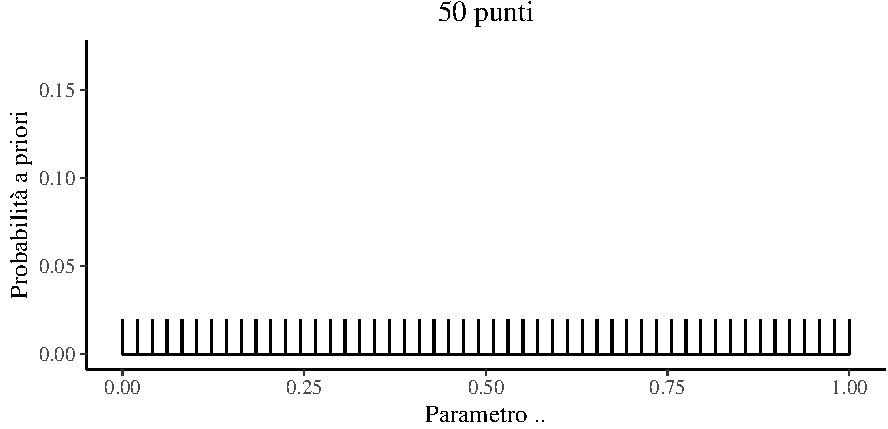
\includegraphics{910_grid_method_example_files/figure-latex/gridappr1-1} 

}

\caption{Rappresentazione grafica della distribuzione a priori per il parametro $   heta$, ovvero la probabilità di aspettative future distorte negativamente.}\label{fig:gridappr1}
\end{figure}

\hypertarget{funzione-di-verosimiglianza}{%
\section{Funzione di verosimiglianza}\label{funzione-di-verosimiglianza}}

Calcoliamo ora la funzione di verosimiglianza utilizzando i 50 valori \(\theta\) definiti in precedenza. A ciascuno dei valori della griglia applichiamo la formula binomiale, tendendo costanti i dati (ovvero 23 ``successi'' in 30 prove). Ad esempio, in corrispondenza del valore \(\theta = 0.816\), l'ordinata della funzione di verosimiglianza diventa

\begin{equation}
\binom{30}{23} \cdot 0.816^{23} \cdot (1 - 0.816)^{7} = 0.135.\notag
\end{equation}

\noindent
Per \(\theta = 0.837\), l'ordinata della funzione di verosimiglianza sarà

\begin{equation}
\binom{30}{23} \cdot 0.837^{23} \cdot (1 - 0.837)^{7} = 0.104.\notag
\end{equation}

\noindent
Dobbiamo svolgere questo calcolo per tutti gli elementi della griglia. Usando \(\R\), tale risultato si trova nel modo seguente:

\begin{Shaded}
\begin{Highlighting}[]
\NormalTok{likelihood }\OtherTok{\textless{}{-}} \FunctionTok{dbinom}\NormalTok{(}\AttributeTok{x =} \DecValTok{23}\NormalTok{, }\AttributeTok{size =} \DecValTok{30}\NormalTok{, }\AttributeTok{prob =}\NormalTok{ p\_grid)}
\NormalTok{likelihood}
\CommentTok{\#\textgreater{}  [1] 0.000000e+00 2.352564e{-}33 1.703051e{-}26 1.644169e{-}22}
\CommentTok{\#\textgreater{}  [5] 1.053708e{-}19 1.525217e{-}17 8.602222e{-}16 2.528440e{-}14}
\CommentTok{\#\textgreater{}  [9] 4.606907e{-}13 5.819027e{-}12 5.499269e{-}11 4.105534e{-}10}
\CommentTok{\#\textgreater{} [13] 2.520191e{-}09 1.311195e{-}08 5.919348e{-}08 2.362132e{-}07}
\CommentTok{\#\textgreater{} [17] 8.456875e{-}07 2.749336e{-}06 8.196948e{-}06 2.259614e{-}05}
\CommentTok{\#\textgreater{} [21] 5.798673e{-}05 1.393165e{-}04 3.148623e{-}04 6.720574e{-}04}
\CommentTok{\#\textgreater{} [25] 1.359225e{-}03 2.611870e{-}03 4.778973e{-}03 8.340230e{-}03}
\CommentTok{\#\textgreater{} [29] 1.390025e{-}02 2.214199e{-}02 3.372227e{-}02 4.909974e{-}02}
\CommentTok{\#\textgreater{} [33] 6.830377e{-}02 9.068035e{-}02 1.146850e{-}01 1.378206e{-}01}
\CommentTok{\#\textgreater{} [37] 1.568244e{-}01 1.681749e{-}01 1.688979e{-}01 1.575211e{-}01}
\CommentTok{\#\textgreater{} [41] 1.348746e{-}01 1.043545e{-}01 7.133007e{-}02 4.165680e{-}02}
\CommentTok{\#\textgreater{} [45] 1.972669e{-}02 6.936821e{-}03 1.535082e{-}03 1.473375e{-}04}
\CommentTok{\#\textgreater{} [49] 1.868105e{-}06 0.000000e+00}
\end{Highlighting}
\end{Shaded}

\noindent
La funzione \texttt{dbinom(x,\ size,\ prob)} richiede che vengano specificati tre parametri: il numero di ``successi'', il numero di prove e la probabilità di successo. Nella chiamata precedente, \texttt{x} (numero di successi) e \texttt{size} (numero di prove bernoulliane) sono degli scalari e \texttt{prob} è il vettore \texttt{p\_grid}. In tali circostanze, l'output di \texttt{dbinom()} è il vettore che abbiamo chiamato \texttt{likelihood}. Gli elementi di tale vettore sono stati calcolati applicando la formula della distribuzione binomiale a ciascuno dei 50 elementi della griglia, tenendo sempre costanti i dati {[}ovvero, \texttt{x} (il numero di successi) e \texttt{size} (numero di prove bernoulliane){]}; ciò che varia è il valore \texttt{prob}, che assume valori diversi (\texttt{p\_grid}) in ciascuna cella della griglia.

La chiamata a \texttt{dbinom()} produce dunque un vettore i cui valori corrispondono all'ordinata della funzione di verosimiglianza per per ciascun valore \(\theta\) specificato in \texttt{p\_grid}. La verosimiglianza discretizzata così ottenuta è riportata nella figura \ref{fig:gridappr2}.

\begin{Shaded}
\begin{Highlighting}[]
\NormalTok{p2 }\OtherTok{\textless{}{-}} \FunctionTok{data.frame}\NormalTok{(p\_grid, likelihood) }\SpecialCharTok{\%\textgreater{}\%}
  \FunctionTok{ggplot}\NormalTok{(}\FunctionTok{aes}\NormalTok{(}\AttributeTok{x =}\NormalTok{ p\_grid, }\AttributeTok{xend =}\NormalTok{ p\_grid, }\AttributeTok{y =} \DecValTok{0}\NormalTok{, }\AttributeTok{yend =}\NormalTok{ likelihood)) }\SpecialCharTok{+}
  \FunctionTok{geom\_segment}\NormalTok{() }\SpecialCharTok{+}
  \FunctionTok{ylim}\NormalTok{(}\DecValTok{0}\NormalTok{, }\FloatTok{0.17}\NormalTok{) }\SpecialCharTok{+}
  \FunctionTok{labs}\NormalTok{(}
    \AttributeTok{x =} \StringTok{"Parametro \textbackslash{}U03B8"}\NormalTok{,}
    \AttributeTok{y =} \StringTok{"Verosimiglianza"}
\NormalTok{  )}
\NormalTok{p2}
\end{Highlighting}
\end{Shaded}

\begin{figure}

{\centering 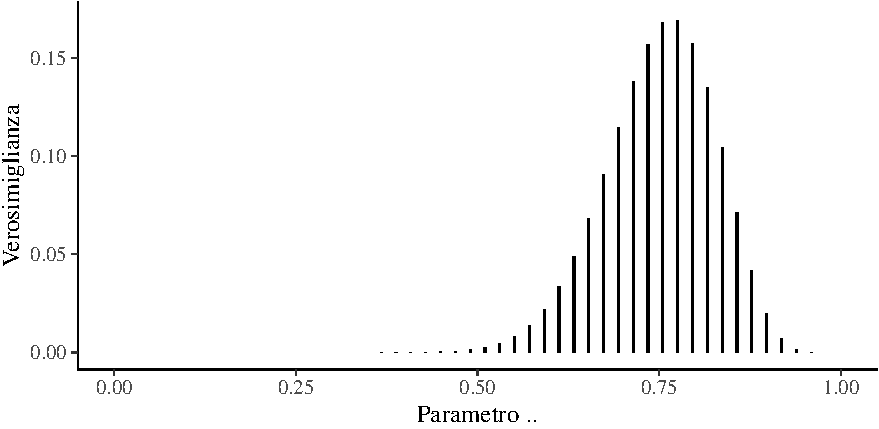
\includegraphics{910_grid_method_example_files/figure-latex/gridappr2-1} 

}

\caption{Rappresentazione della funzione di verosimiglianza per il parametro $\theta$, ovvero la probabilità di aspettative future distorte negativamente.}\label{fig:gridappr2}
\end{figure}

\hypertarget{distribuzione-a-posteriori}{%
\section{Distribuzione a posteriori}\label{distribuzione-a-posteriori}}

L'approssimazione discretizzata della distribuzione a posteriori \(p(\theta \mid y)\) si ottiene facendo il prodotto della verosimiglianza e della distribuzione a priori per poi scalare tale prodotto per una costante di normalizzazione. Il prodotto \(p(\theta)\mathcal{L}(y \mid \theta)\) produce la distribuzione a posteriori \emph{non standardizzata}.

Nel caso di una distribuzione a priori non informativa (ovvero una distribuzione uniforme), per ottenere la funzione a posteriori non standardizzata è sufficiente moltiplicare ciascun valore della funzione di verosimiglianza per 0.02. Per esempio, per il primo valore della funzione di verosimiglianza usato quale esempio poco sopra, abbiamo \(0.135 \cdot 0.02\); per il secondo valore dell'esempio abbiamo \(0.104 \cdot 0.02\); e così via. Possiamo svolgere tutti i calcoli usando \(\R\) nel modo seguente:\footnote{Ricordiamo il principio dell'aritmetica vettorializzata: i vettori \texttt{likelihood} e \texttt{prior1} sono entrambi costituiti da 50 elementi. Se facciamo il prodotto tra i due vettori otteniamo un vettore di 50 elementi, ciascuno dei quali uguale al prodotto dei corrispondenti elementi dei vettori \texttt{likelihood} e \texttt{prior1}.}

\begin{Shaded}
\begin{Highlighting}[]
\NormalTok{unstd\_posterior }\OtherTok{\textless{}{-}}\NormalTok{ likelihood }\SpecialCharTok{*}\NormalTok{ prior1}
\NormalTok{unstd\_posterior}
\CommentTok{\#\textgreater{}  [1] 0.000000e+00 4.705127e{-}35 3.406102e{-}28 3.288337e{-}24}
\CommentTok{\#\textgreater{}  [5] 2.107415e{-}21 3.050433e{-}19 1.720444e{-}17 5.056880e{-}16}
\CommentTok{\#\textgreater{}  [9] 9.213813e{-}15 1.163805e{-}13 1.099854e{-}12 8.211068e{-}12}
\CommentTok{\#\textgreater{} [13] 5.040382e{-}11 2.622390e{-}10 1.183870e{-}09 4.724263e{-}09}
\CommentTok{\#\textgreater{} [17] 1.691375e{-}08 5.498671e{-}08 1.639390e{-}07 4.519229e{-}07}
\CommentTok{\#\textgreater{} [21] 1.159735e{-}06 2.786331e{-}06 6.297247e{-}06 1.344115e{-}05}
\CommentTok{\#\textgreater{} [25] 2.718450e{-}05 5.223741e{-}05 9.557946e{-}05 1.668046e{-}04}
\CommentTok{\#\textgreater{} [29] 2.780049e{-}04 4.428398e{-}04 6.744454e{-}04 9.819948e{-}04}
\CommentTok{\#\textgreater{} [33] 1.366075e{-}03 1.813607e{-}03 2.293700e{-}03 2.756411e{-}03}
\CommentTok{\#\textgreater{} [37] 3.136488e{-}03 3.363497e{-}03 3.377958e{-}03 3.150422e{-}03}
\CommentTok{\#\textgreater{} [41] 2.697491e{-}03 2.087091e{-}03 1.426601e{-}03 8.331361e{-}04}
\CommentTok{\#\textgreater{} [45] 3.945339e{-}04 1.387364e{-}04 3.070164e{-}05 2.946751e{-}06}
\CommentTok{\#\textgreater{} [49] 3.736209e{-}08 0.000000e+00}
\end{Highlighting}
\end{Shaded}

Avendo calcolato i valori della funzione a posteriori non standardizzata è poi necessario dividere per una costante di normalizzazione. Nel caso discreto, trovare il denominatore del teorema di Bayes è facile: esso è uguale alla somma di tutti i valori della distribuzione a posteriori non normalizzata. Per i dati presenti, tale costante di normalizzazione è uguale a 0.032:

\begin{Shaded}
\begin{Highlighting}[]
\FunctionTok{sum}\NormalTok{(unstd\_posterior)}
\CommentTok{\#\textgreater{} [1] 0.0316129}
\end{Highlighting}
\end{Shaded}

La standardizzazione dei due valori usati come esempio è data da: \(0.135 \cdot 0.02 / 0.032\) e da \(0.104 \cdot 0.02 / 0.032\). Usiamo \(\R\) per svolgere questo calcolo su tutti i 50 valori di \texttt{unstd\_posterior} così che la somma dei 50 i valori di \texttt{posterior} sia uguale a 1.0:

\begin{Shaded}
\begin{Highlighting}[]
\NormalTok{posterior }\OtherTok{\textless{}{-}}\NormalTok{ unstd\_posterior }\SpecialCharTok{/} \FunctionTok{sum}\NormalTok{(unstd\_posterior)}
\NormalTok{posterior}
\CommentTok{\#\textgreater{}  [1] 0.000000e+00 1.488357e{-}33 1.077440e{-}26 1.040188e{-}22}
\CommentTok{\#\textgreater{}  [5] 6.666313e{-}20 9.649330e{-}18 5.442222e{-}16 1.599625e{-}14}
\CommentTok{\#\textgreater{}  [9] 2.914574e{-}13 3.681425e{-}12 3.479129e{-}11 2.597379e{-}10}
\CommentTok{\#\textgreater{} [13] 1.594406e{-}09 8.295316e{-}09 3.744893e{-}08 1.494410e{-}07}
\CommentTok{\#\textgreater{} [17] 5.350268e{-}07 1.739376e{-}06 5.185824e{-}06 1.429552e{-}05}
\CommentTok{\#\textgreater{} [21] 3.668548e{-}05 8.813904e{-}05 1.991986e{-}04 4.251792e{-}04}
\CommentTok{\#\textgreater{} [25] 8.599178e{-}04 1.652408e{-}03 3.023432e{-}03 5.276472e{-}03}
\CommentTok{\#\textgreater{} [29] 8.794033e{-}03 1.400820e{-}02 2.133450e{-}02 3.106310e{-}02}
\CommentTok{\#\textgreater{} [33] 4.321259e{-}02 5.736920e{-}02 7.255582e{-}02 8.719259e{-}02}
\CommentTok{\#\textgreater{} [37] 9.921545e{-}02 1.063963e{-}01 1.068538e{-}01 9.965619e{-}02}
\CommentTok{\#\textgreater{} [41] 8.532881e{-}02 6.602021e{-}02 4.512719e{-}02 2.635430e{-}02}
\CommentTok{\#\textgreater{} [45] 1.248015e{-}02 4.388601e{-}03 9.711744e{-}04 9.321354e{-}05}
\CommentTok{\#\textgreater{} [49] 1.181862e{-}06 0.000000e+00}
\end{Highlighting}
\end{Shaded}

\noindent 
Verifichiamo:

\begin{Shaded}
\begin{Highlighting}[]
\FunctionTok{sum}\NormalTok{(posterior)}
\CommentTok{\#\textgreater{} [1] 1}
\end{Highlighting}
\end{Shaded}

La distribuzione a posteriori così trovata non è altro che la versione normalizzata della funzione di verosimiglianza: questo avviene perché la distribuzione a priori uniforme non ha aggiunto altre informazioni oltre a quelle che erano già fornite dalla funzione di verosimiglianza. L'approssimazione discretizzata di \(p(\theta \mid y)\) che abbiamo appena trovato è riportata nella figura \ref{fig:gridappr3}.

\begin{Shaded}
\begin{Highlighting}[]
\NormalTok{p3 }\OtherTok{\textless{}{-}} \FunctionTok{data.frame}\NormalTok{(p\_grid, posterior) }\SpecialCharTok{\%\textgreater{}\%}
  \FunctionTok{ggplot}\NormalTok{(}\FunctionTok{aes}\NormalTok{(}\AttributeTok{x =}\NormalTok{ p\_grid, }\AttributeTok{xend =}\NormalTok{ p\_grid, }\AttributeTok{y =} \DecValTok{0}\NormalTok{, }\AttributeTok{yend =}\NormalTok{ posterior)) }\SpecialCharTok{+}
  \FunctionTok{geom\_segment}\NormalTok{() }\SpecialCharTok{+}
  \FunctionTok{ylim}\NormalTok{(}\DecValTok{0}\NormalTok{, }\FloatTok{0.17}\NormalTok{) }\SpecialCharTok{+}
  \FunctionTok{labs}\NormalTok{(}
    \AttributeTok{x =} \StringTok{"Parametro \textbackslash{}U03B8"}\NormalTok{,}
    \AttributeTok{y =} \StringTok{"Probabilità a posteriori"}
\NormalTok{  )}
\NormalTok{p3}
\end{Highlighting}
\end{Shaded}

\begin{figure}

{\centering 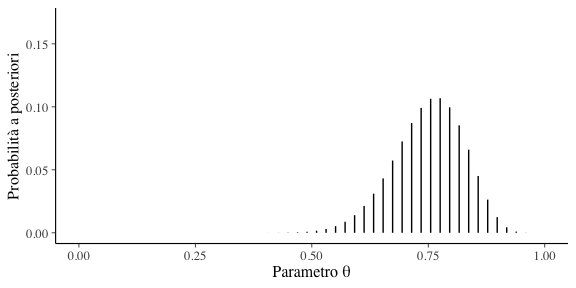
\includegraphics{910_grid_method_example_files/figure-latex/gridappr3-1} 

}

\caption{Rappresentazione della distribuzione a posteriori per il parametro $\theta$, ovvero la probabilità di aspettative future distorte negativamente.}\label{fig:gridappr3}
\end{figure}

I grafici delle figure \ref{fig:gridappr1}, \ref{fig:gridappr2} e \ref{fig:gridappr3} sono state calcolati utilizzando una griglia di 50 valori equi-spaziati per il parametro \(\theta\). I segmenti verticali rappresentano l'intensità della funzione in corrispondenza di ciascuna modalità parametro \(\theta\). Nella figura \ref{fig:gridappr1} e nella figura \ref{fig:gridappr3} la somma delle lunghezze dei segmenti verticali è uguale a 1.0; ciò non si verifica, invece, nel caso della figura \ref{fig:gridappr3} (la funzione di verosimiglianza non è mai una funzione di probabilità, né nel caso discreto né in quello continuo).

\hypertarget{es-depression-beta-2-10}{%
\section{La stima della distribuzione a posteriori (versione 2)}\label{es-depression-beta-2-10}}

Continuiamo l'analisi di questi dati esaminiamo l'impatto di una distribuzione a priori informativa sulla distribuzione a posteriori. Una distribuzione a priori informativa riflette un alto grado di certezza a priori sui valori dei parametri del modello. Un ricercatore utilizza una distribuzione a priori informativa per introdurre nel processo di stima informazioni pre-esistenti alla raccolta dei dati, introducendo così delle restrizioni sulla possibile gamma di valori del parametro.

Nel caso presente, supponiamo che la letteratura psicologica fornisca delle informazioni su \(\theta\) (la probabilità che le aspettative future di un individuo clinicamente depresso siano distorte negativamente). Per fare un esempio, supponiamo (irrealisticamente) che tali conoscenze pregresse possano essere rappresentate da una Beta di parametri \(\alpha = 2\) e \(\beta = 10\). Tali ipotetiche conoscenze pregresse ritengono molto plausibili valori \(\theta\) bassi e considerano implausibili valori \(\theta > 0.5\). Questo è equivalente a dire che ci aspettiamo che le aspettative relative all'umore futuro siano distorte negativamente solo per pochissimi individui clinicamente depressi --- ovvero, ci aspettiamo che la maggioranza degli individui clinicamente depressi sia inguaribilmente ottimista. Questa è, ovviamente, una credenza a priori del tutto irrealistica. La esamino qui, non perché abbia alcun senso nel contesto dei dati di \citet{zetschefuture2019}, ma soltanto per fare un esempio nel quale risulta chiaro come la distribuzione a posteriori sia una sorta di ``compromesso'' tra la distribuzione a priori e la verosimiglianza.

Con calcoli del tutto simili a quelli descritti sopra si giunge alla distribuzione a posteriori rappresentata nella figura \ref{fig:gridappr4}. Useremo ora una griglia di 100 valori per il parametro \(\theta\):

\begin{Shaded}
\begin{Highlighting}[]
\NormalTok{n\_points }\OtherTok{\textless{}{-}} \DecValTok{100}
\NormalTok{p\_grid }\OtherTok{\textless{}{-}} \FunctionTok{seq}\NormalTok{(}\AttributeTok{from =} \DecValTok{0}\NormalTok{, }\AttributeTok{to =} \DecValTok{1}\NormalTok{, }\AttributeTok{length.out =}\NormalTok{ n\_points)}
\end{Highlighting}
\end{Shaded}

\noindent
Per la distribuzione a priori scegliamo una Beta(2, 10):

\begin{Shaded}
\begin{Highlighting}[]
\NormalTok{alpha }\OtherTok{\textless{}{-}} \DecValTok{2}
\NormalTok{beta }\OtherTok{\textless{}{-}} \DecValTok{10}
\NormalTok{prior2 }\OtherTok{\textless{}{-}} \FunctionTok{dbeta}\NormalTok{(p\_grid, alpha, beta) }\SpecialCharTok{/} \FunctionTok{sum}\NormalTok{(}\FunctionTok{dbeta}\NormalTok{(p\_grid, alpha, beta))}
\FunctionTok{sum}\NormalTok{(prior2)}
\CommentTok{\#\textgreater{} [1] 1}
\end{Highlighting}
\end{Shaded}

\noindent
Tale distribuzione a priori è rappresentata nella figura \ref{fig:gridappr4}:

\begin{Shaded}
\begin{Highlighting}[]
\NormalTok{plot\_df }\OtherTok{\textless{}{-}} \FunctionTok{data.frame}\NormalTok{(p\_grid, prior2)}
\NormalTok{p4 }\OtherTok{\textless{}{-}}\NormalTok{ plot\_df }\SpecialCharTok{\%\textgreater{}\%}
  \FunctionTok{ggplot}\NormalTok{(}\FunctionTok{aes}\NormalTok{(}\AttributeTok{x =}\NormalTok{ p\_grid, }\AttributeTok{xend =}\NormalTok{ p\_grid, }\AttributeTok{y =} \DecValTok{0}\NormalTok{, }\AttributeTok{yend =}\NormalTok{ prior2)) }\SpecialCharTok{+}
  \FunctionTok{geom\_segment}\NormalTok{() }\SpecialCharTok{+}
  \FunctionTok{ylim}\NormalTok{(}\DecValTok{0}\NormalTok{, }\FloatTok{0.17}\NormalTok{) }\SpecialCharTok{+}
  \FunctionTok{labs}\NormalTok{(}
    \AttributeTok{x =} \StringTok{""}\NormalTok{,}
    \AttributeTok{y =} \StringTok{"Probabilità a priori"}
\NormalTok{  )}
\NormalTok{p4}
\end{Highlighting}
\end{Shaded}

\begin{figure}

{\centering 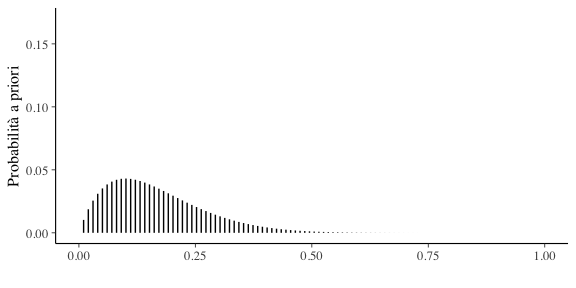
\includegraphics{910_grid_method_example_files/figure-latex/gridappr4-1} 

}

\caption{Rappresentazione di una funzione a priori informativa per il parametro $\theta$.}\label{fig:gridappr4}
\end{figure}

\noindent
Calcoliamo il valore di verosimiglianza per ciascun punto della griglia:

\begin{Shaded}
\begin{Highlighting}[]
\NormalTok{likelihood }\OtherTok{\textless{}{-}} \FunctionTok{dbinom}\NormalTok{(}\DecValTok{23}\NormalTok{, }\AttributeTok{size =} \DecValTok{30}\NormalTok{, }\AttributeTok{prob =}\NormalTok{ p\_grid)}
\end{Highlighting}
\end{Shaded}

\noindent
Per ciascun punto della griglia, il prodotto tra la verosimiglianza e distribuzione a priori è dato da:

\begin{Shaded}
\begin{Highlighting}[]
\NormalTok{unstd\_posterior2 }\OtherTok{\textless{}{-}}\NormalTok{ likelihood }\SpecialCharTok{*}\NormalTok{ prior2}
\end{Highlighting}
\end{Shaded}

\noindent
È necessario normalizzare la distribuzione a posteriori discretizzata:

\begin{Shaded}
\begin{Highlighting}[]
\NormalTok{posterior2 }\OtherTok{\textless{}{-}}\NormalTok{ unstd\_posterior2 }\SpecialCharTok{/} \FunctionTok{sum}\NormalTok{(unstd\_posterior2)}
\end{Highlighting}
\end{Shaded}

\noindent
Verifichiamo:

\begin{Shaded}
\begin{Highlighting}[]
\FunctionTok{sum}\NormalTok{(posterior2)}
\CommentTok{\#\textgreater{} [1] 1}
\end{Highlighting}
\end{Shaded}

\noindent
La nuova funzione a posteriori discretizzata è rappresentata nella figura \ref{fig:gridappr5}:

\begin{Shaded}
\begin{Highlighting}[]
\NormalTok{plot\_df }\OtherTok{\textless{}{-}} \FunctionTok{data.frame}\NormalTok{(p\_grid, posterior2)}
\NormalTok{p5 }\OtherTok{\textless{}{-}}\NormalTok{ plot\_df }\SpecialCharTok{\%\textgreater{}\%}
  \FunctionTok{ggplot}\NormalTok{(}\FunctionTok{aes}\NormalTok{(}\AttributeTok{x =}\NormalTok{ p\_grid, }\AttributeTok{xend =}\NormalTok{ p\_grid, }\AttributeTok{y =} \DecValTok{0}\NormalTok{, }\AttributeTok{yend =}\NormalTok{ posterior2)) }\SpecialCharTok{+}
  \FunctionTok{geom\_segment}\NormalTok{() }\SpecialCharTok{+}
  \FunctionTok{ylim}\NormalTok{(}\DecValTok{0}\NormalTok{, }\FloatTok{0.17}\NormalTok{) }\SpecialCharTok{+}
  \FunctionTok{labs}\NormalTok{(}
    \AttributeTok{x =} \StringTok{"Parametro \textbackslash{}U03B8"}\NormalTok{,}
    \AttributeTok{y =} \StringTok{"Probabilità a posteriori"}
\NormalTok{  )}
\NormalTok{p5}
\end{Highlighting}
\end{Shaded}

\begin{figure}

{\centering 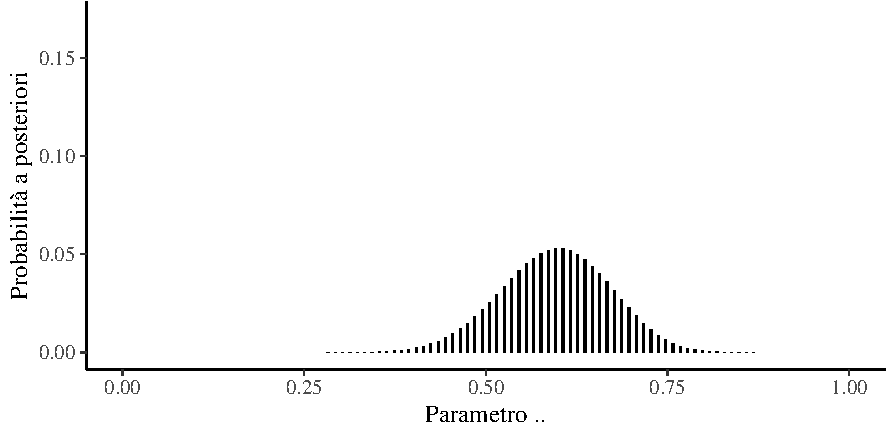
\includegraphics{910_grid_method_example_files/figure-latex/gridappr5-1} 

}

\caption{Rappresentazione della funzione a posteriori per il parametro $\theta$ calcolata utilizzando una distribuzione a priori informativa.}\label{fig:gridappr5}
\end{figure}

Facendo un confronto tra le figure \ref{fig:gridappr4} e \ref{fig:gridappr5} notiamo una notevole differenza tra la distribuzione a priori e la distribuzione a posteriori. In particolare, la distribuzione a posteriori risulta spostata verso destra su posizioni più vicine a quelle della verosimiglianza {[}figura \ref{fig:gridappr2}{]}. Si noti inoltre che, a causa dell'effetto della distribuzione a priori, le distribuzioni a posteriori delle figure \ref{fig:gridappr3} e \ref{fig:gridappr5} sono molto diverse tra loro.

Campioniamo ora 10,000 punti dall'approssimazione discretizzata della distribuzione a posteriori:

\begin{Shaded}
\begin{Highlighting}[]
\CommentTok{\# Set the seed}
\FunctionTok{set.seed}\NormalTok{(}\DecValTok{84735}\NormalTok{)}

\NormalTok{df }\OtherTok{\textless{}{-}} \FunctionTok{data.frame}\NormalTok{(}
\NormalTok{  p\_grid,}
\NormalTok{  posterior2}
\NormalTok{)}
\CommentTok{\# Step 4: sample from the discretized posterior}
\NormalTok{post\_samples }\OtherTok{\textless{}{-}}\NormalTok{ df }\SpecialCharTok{\%\textgreater{}\%}
  \FunctionTok{slice\_sample}\NormalTok{(}
    \AttributeTok{n =} \FloatTok{1e5}\NormalTok{,}
    \AttributeTok{weight\_by =}\NormalTok{ posterior2,}
    \AttributeTok{replace =} \ConstantTok{TRUE}
\NormalTok{  )}
\end{Highlighting}
\end{Shaded}

\noindent
Una rappresentazione grafica del campione casuale estratto dalla distribuzione a posteriori \(p(\theta \mid y)\) è data da:

\begin{Shaded}
\begin{Highlighting}[]
\NormalTok{post\_samples }\SpecialCharTok{\%\textgreater{}\%}
  \FunctionTok{ggplot}\NormalTok{(}\FunctionTok{aes}\NormalTok{(}\AttributeTok{x =}\NormalTok{ p\_grid)) }\SpecialCharTok{+}
  \FunctionTok{geom\_histogram}\NormalTok{(}
    \FunctionTok{aes}\NormalTok{(}\AttributeTok{y =}\NormalTok{ ..density..),}
    \AttributeTok{color =} \StringTok{"white"}\NormalTok{,}
    \AttributeTok{binwidth =} \FloatTok{0.05}
\NormalTok{  ) }\SpecialCharTok{+}
  \FunctionTok{stat\_function}\NormalTok{(}\AttributeTok{fun =}\NormalTok{ dbeta, }\AttributeTok{args =} \FunctionTok{list}\NormalTok{(}\DecValTok{25}\NormalTok{, }\DecValTok{17}\NormalTok{)) }\SpecialCharTok{+}
  \FunctionTok{lims}\NormalTok{(}\AttributeTok{x =} \FunctionTok{c}\NormalTok{(}\DecValTok{0}\NormalTok{, }\DecValTok{1}\NormalTok{))}
\end{Highlighting}
\end{Shaded}

\begin{center}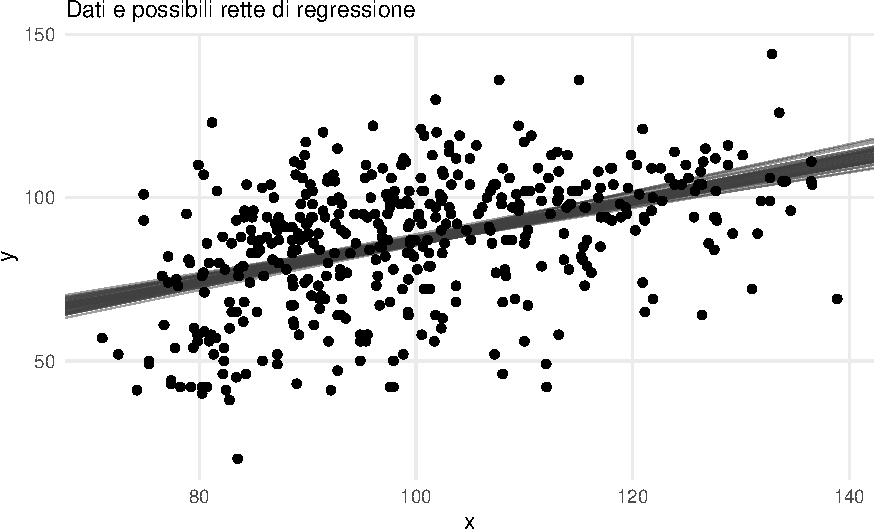
\includegraphics{910_grid_method_example_files/figure-latex/unnamed-chunk-16-1} \end{center}

\noindent
All'istogramma è stata sovrapposta la corretta distribuzione a posteriori, ovvero una Beta di parametri 25 (\(y + \alpha\) = 23 + 2) e 17 (\(n - y + \beta\) = 30 - 23 + 10).

La stima della moda a posteriori si ottiene con

\begin{Shaded}
\begin{Highlighting}[]
\NormalTok{df}\SpecialCharTok{$}\NormalTok{p\_grid[}\FunctionTok{which.max}\NormalTok{(df}\SpecialCharTok{$}\NormalTok{posterior2)]}
\CommentTok{\#\textgreater{} [1] 0.5959596}
\end{Highlighting}
\end{Shaded}

\noindent e corrisponde a

\[
\Mo = \frac{\alpha -1}{\alpha + \beta - 2} = \frac{25 - 1}{25 + 17 - 2} = 0.6.
\]

La stima della media a posteriori si ottiene con

\begin{Shaded}
\begin{Highlighting}[]
\FunctionTok{mean}\NormalTok{(post\_samples}\SpecialCharTok{$}\NormalTok{p\_grid)}
\CommentTok{\#\textgreater{} [1] 0.5953337}
\end{Highlighting}
\end{Shaded}

\noindent e corrisponde a

\[
\bar{\theta} = \frac{\alpha}{\alpha + \beta} = \frac{25}{25 + 17} \approx 0.5952.
\]

La stima della mediana a posteriori si ottiene con

\begin{Shaded}
\begin{Highlighting}[]
\FunctionTok{median}\NormalTok{(post\_samples}\SpecialCharTok{$}\NormalTok{p\_grid)}
\CommentTok{\#\textgreater{} [1] 0.5959596}
\end{Highlighting}
\end{Shaded}

\noindent e corrisponde a

\[
\Me = \frac{\alpha - \frac{1}{3}}{\alpha + \beta - \frac{2}{3}} \approx 0.5968.
\]

\hypertarget{es-pratico-zetsche-funzioni}{%
\section{Versione 2}\label{es-pratico-zetsche-funzioni}}

Possiamo semplificare i calcoli precedenti definendo le funzioni \texttt{likelihood()}, \texttt{prior()} e \texttt{posterior()}.

Per calcolare la funzione di verosimiglianza per i 30 valori di \citet{zetschefuture2019} useremo la funzione \texttt{likelihood()}:

\begin{Shaded}
\begin{Highlighting}[]
\NormalTok{x }\OtherTok{\textless{}{-}} \DecValTok{23}
\NormalTok{N }\OtherTok{\textless{}{-}} \DecValTok{30}
\NormalTok{param }\OtherTok{\textless{}{-}} \FunctionTok{seq}\NormalTok{(}\DecValTok{0}\NormalTok{, }\DecValTok{1}\NormalTok{, }\AttributeTok{length.out =} \DecValTok{100}\NormalTok{)}

\NormalTok{likelihood }\OtherTok{\textless{}{-}} \ControlFlowTok{function}\NormalTok{(param, }\AttributeTok{x =} \DecValTok{23}\NormalTok{, }\AttributeTok{N =} \DecValTok{30}\NormalTok{) \{}
  \FunctionTok{dbinom}\NormalTok{(x, N, param)}
\NormalTok{\}}

\FunctionTok{tibble}\NormalTok{(}
  \AttributeTok{x =}\NormalTok{ param,}
  \AttributeTok{y =} \FunctionTok{likelihood}\NormalTok{(param)}
\NormalTok{) }\SpecialCharTok{\%\textgreater{}\%}
  \FunctionTok{ggplot}\NormalTok{(}\FunctionTok{aes}\NormalTok{(x, y)) }\SpecialCharTok{+}
  \FunctionTok{geom\_line}\NormalTok{() }\SpecialCharTok{+}
  \FunctionTok{labs}\NormalTok{(}
    \AttributeTok{x =} \FunctionTok{expression}\NormalTok{(theta),}
    \AttributeTok{y =} \StringTok{"Verosimiglianza"}
\NormalTok{  )}
\end{Highlighting}
\end{Shaded}

\begin{center}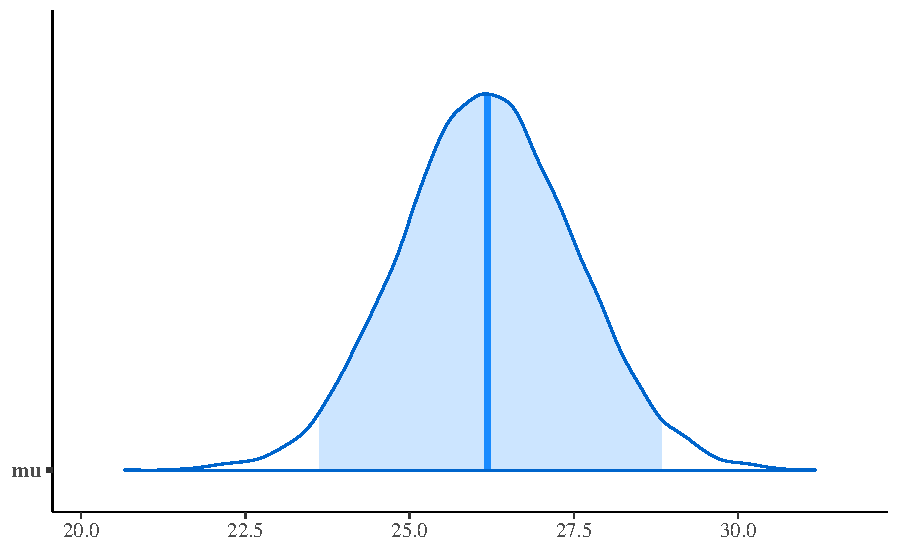
\includegraphics{910_grid_method_example_files/figure-latex/unnamed-chunk-20-1} \end{center}

\noindent
La funzione \texttt{likelihood()} ritorna l'ordinata della verosimiglianza binomiale per ciascun valore del vettore \texttt{param} in input.

Quale distribuzione a priori utilizzeremo una \(\mbox{Beta}(2, 10)\) che è implementata nella funzione \texttt{prior()}:

\begin{Shaded}
\begin{Highlighting}[]
\NormalTok{prior }\OtherTok{\textless{}{-}} \ControlFlowTok{function}\NormalTok{(param, }\AttributeTok{alpha =} \DecValTok{2}\NormalTok{, }\AttributeTok{beta =} \DecValTok{10}\NormalTok{) \{}
\NormalTok{  param\_vals }\OtherTok{\textless{}{-}} \FunctionTok{seq}\NormalTok{(}\DecValTok{0}\NormalTok{, }\DecValTok{1}\NormalTok{, }\AttributeTok{length.out =} \DecValTok{100}\NormalTok{)}
  \FunctionTok{dbeta}\NormalTok{(param, alpha, beta) }\CommentTok{\# / sum(dbeta(param\_vals, alpha, beta))}
\NormalTok{\}}

\FunctionTok{tibble}\NormalTok{(}
  \AttributeTok{x =}\NormalTok{ param,}
  \AttributeTok{y =} \FunctionTok{prior}\NormalTok{(param)}
\NormalTok{) }\SpecialCharTok{\%\textgreater{}\%}
  \FunctionTok{ggplot}\NormalTok{(}\FunctionTok{aes}\NormalTok{(x, y)) }\SpecialCharTok{+}
  \FunctionTok{geom\_line}\NormalTok{() }\SpecialCharTok{+}
  \FunctionTok{labs}\NormalTok{(}
    \AttributeTok{x =} \FunctionTok{expression}\NormalTok{(theta),}
    \AttributeTok{y =} \StringTok{"Densità"}
\NormalTok{  )}
\end{Highlighting}
\end{Shaded}

\begin{center}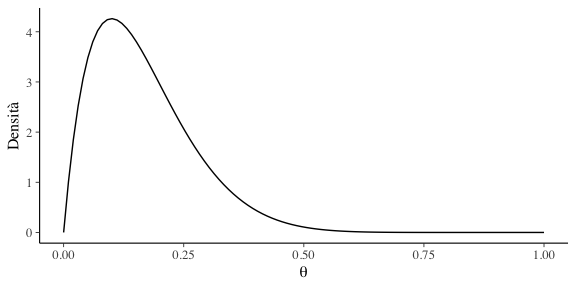
\includegraphics{910_grid_method_example_files/figure-latex/unnamed-chunk-21-1} \end{center}

La funzione \texttt{posterior()} ritorna il prodotto della densità a priori e della verosimiglianza:

\begin{Shaded}
\begin{Highlighting}[]
\NormalTok{posterior }\OtherTok{\textless{}{-}} \ControlFlowTok{function}\NormalTok{(param) \{}
  \FunctionTok{likelihood}\NormalTok{(param) }\SpecialCharTok{*} \FunctionTok{prior}\NormalTok{(param)}
\NormalTok{\}}

\FunctionTok{tibble}\NormalTok{(}
  \AttributeTok{x =}\NormalTok{ param,}
  \AttributeTok{y =} \FunctionTok{posterior}\NormalTok{(param)}
\NormalTok{) }\SpecialCharTok{\%\textgreater{}\%}
  \FunctionTok{ggplot}\NormalTok{(}\FunctionTok{aes}\NormalTok{(x, y)) }\SpecialCharTok{+}
  \FunctionTok{geom\_line}\NormalTok{() }\SpecialCharTok{+}
  \FunctionTok{labs}\NormalTok{(}
    \AttributeTok{x =} \FunctionTok{expression}\NormalTok{(theta),}
    \AttributeTok{y =} \StringTok{"Densità"}
\NormalTok{  )}
\end{Highlighting}
\end{Shaded}

\begin{center}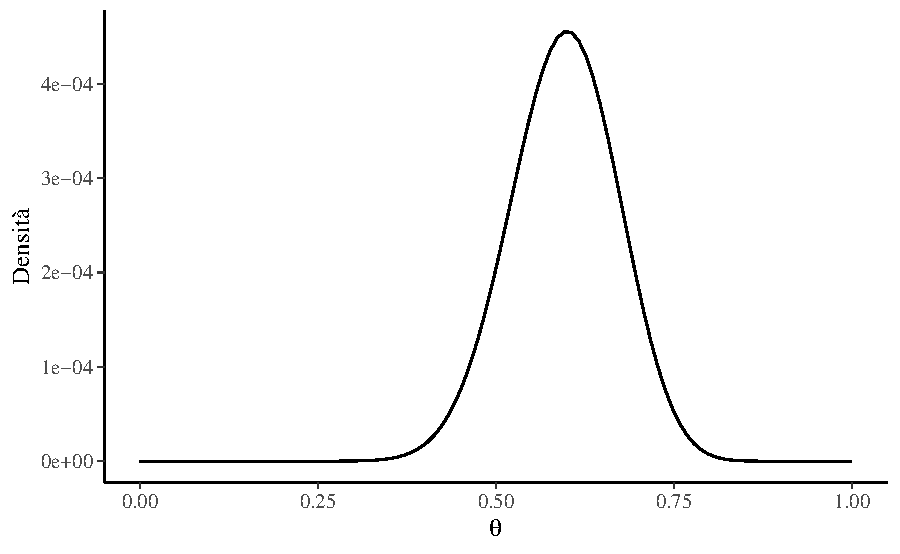
\includegraphics{910_grid_method_example_files/figure-latex/unnamed-chunk-22-1} \end{center}

\noindent
La distribuzione a posteriori non normalizzata mostrata nella figura replica il risultato ottenuto con il codice utilizzato nella prima parte di questo Capitolo. Per l'implementazione dell'algoritmo di Metropolis non è necessaria la normalizzazione della distribuzione a posteriori.

\hypertarget{integration-mc}{%
\chapter{Integrazione di Monte Carlo}\label{integration-mc}}

Il termine Monte Carlo si riferisce al fatto che la computazione fa ricorso ad un ripetuto campionamento casuale attraverso la generazione di sequenze di numeri casuali. Una delle sue applicazioni più potenti è il calcolo degli integrali mediante simulazione numerica. Sia l'integrale da calcolare

\[
\int_a^b h(y) dy.
\]
Se decomponiamo \(h(y)\) nel prodotto di una funzione \(f(y)\) e una funzione di densità
di probabilità \(p(y)\) definita nell'intervallo \((a, b)\) avremo:

\[
\int_a^b h(y) dy = \int_a^b f(y) p(y) dy = \E[f(y)],
\]
così che l'integrale può essere espresso come una funzione di aspettazione \(f(y)\) sulla densità \(p(y)\). Se definiamo un gran numero di variabili casuali \(y_1, y_2, \dots, y_n\) appartenenti alla densità di probabilità \(p(y)\) allora avremo

\[
\int_a^b h(y) dy = \int_a^b f(y) p(y) dy = \E[f(y)] \approx \frac{1}{n}\sum_{i=1}^n f(y)
\]
che è l'integrale di Monte Carlo.

L'integrazione con metodo Monte Carlo trova la sua giustificazione nella \emph{Legge forte dei grandi numeri}. Data una successione di variabili casuali \(Y_{1}, Y_{2},\dots, Y_{n},\dots\) indipendenti e identicamente distribuite con media \(\mu\), ne segue che

\[
P\left( \lim_{n \rightarrow \infty} \frac{1}{n} \sum_{i=1}^n Y_i = \mu \right) = 1.
\]
Ciò significa che, al crescere di \(n\), la media delle realizzazioni di \(Y_{1}, Y_{2},\dots, Y_{n},\dots\) converge con probabilità 1 al vero valore \(\mu\).

Possiamo fornire un esempio intuitivo della legge forte dei grandi numeri facendo riferimento ad una serie di lanci di una moneta dove \(Y=1\) significa ``testa'' e \(Y=0\) significa ``croce''. Per la legge forte dei grandi numeri, nel caso di una moneta equilibrata la proporzione di eventi ``testa'' converge alla vera probabilità dell'evento ``testa''

\[
  \frac{1}{n} \sum_{i=1}^n Y_i \rightarrow \frac{1}{2}
\]
con probabilità di uno.

Quello che è stato detto sopra non è che un modo sofisticato per dire che, se vogliamo calcolare un'approssimazione del valore atteso di una variabile casuale, non dobbiamo fare altro che la media aritmetica di un grande numero di realizzazioni della variabile casuale. Come è facile intuire, l'approssimazione migliora al crescere del numero di dati che abbiamo a disposizione.

L'integrazione di Monte Carlo può essere usata per approssimare la distribuzione a posteriori richiesta da una analisi Bayesiana: una stima di \(p(\theta \mid y)\) può essere ottenuta mediante un grande numero di campioni casuali della distribuzionea a posteriori.

\hypertarget{intro-stan}{%
\chapter{Programmare in Stan}\label{intro-stan}}

\hypertarget{che-cosuxe8-stan}{%
\section{Che cos'è Stan?}\label{che-cosuxe8-stan}}

\href{http://mc-stan.org/}{STAN} è un linguaggio di programmazione probabilistico usato per l'inferenza bayesiana \citep{carpenter2017stan}. Prende il nome da uno dei creatori del metodo Monte Carlo, Stanislaw Ulam \citep{Eckhardt1987stan}. Stan consente di generare campioni da distribuzioni di probabilità basati sulla costruzione di una catena di Markov avente come distribuzione di equilibrio (o stazionaria) la distribuzione desiderata.

Nelle parole degli autori:

\begin{quote}
Stan is a state-of-the-art platform for statistical modeling and high-performance statistical computation. Thousands of users rely on Stan for statistical modeling, data analysis, and prediction in the social, biological, and physical sciences, engineering, and business. Users specify log density functions in Stan's probabilistic programming language and get: full Bayesian statistical inference with MCMC sampling (NUTS, HMC); approximate Bayesian inference with variational inference (ADVI): penalized maximum likelihood estimation with optimization (L-BFGS).
\end{quote}

È possibile accedere al linguaggio Stan tramite diverse interfacce:

\begin{itemize}
\tightlist
\item
  \texttt{CmdStan}: eseguibile da riga di comando,
\item
  \texttt{RStan} - integrazione con il linguaggio \R;
\item
  \texttt{PyStan} - integrazione con il linguaggio di programmazione Python;
\item
  \texttt{MatlabStan} - integrazione con MATLAB;
\item
  \texttt{Stan.jl} - integrazione con il linguaggio di programmazione Julia;
\item
  \texttt{StataStan} - integrazione con Stata.
\end{itemize}

Inoltre, vengono fornite interfacce di livello superiore con i pacchetti che utilizzano Stan come backend, principalmente in Linguaggio \R:

\begin{itemize}
\tightlist
\item
  \texttt{shinystan}: interfaccia grafica interattiva per l'analisi della distribuzione a posteriori e le diagnostiche MCMC;\\
\item
  \texttt{bayesplot}: insieme di funzioni utilizzabili per creare grafici relativi all'analisi della distribuzione a posteriori, ai test del modello e alle diagnostiche MCMC;\\
\item
  \texttt{brms}: fornisce un'ampia gamma di modelli lineari e non lineari specificando i modelli statistici mediante la sintassi usata in \R;
\item
  \texttt{rstanarm}: fornisce un sostituto per i modelli frequentisti forniti da base \(\R\) e \texttt{lme4} utilizzando la sintassi usata in \(\R\) per la specificazione dei modelli statistici;
\item
  \texttt{edstan}: modelli Stan per la Item Response Theory;
\item
  \texttt{cmdstanr}, un'interfaccia \(\R\) per \texttt{CmdStan}.
\end{itemize}

\hypertarget{interfaccia-cmdstanr}{%
\section{\texorpdfstring{Interfaccia \texttt{cmdstanr}}{Interfaccia cmdstanr}}\label{interfaccia-cmdstanr}}

Negli esempi di questa dispensa verrà usata l'interfaccia \texttt{cmdstanr}. Il pacchetto \texttt{cmdstanr} non è ancora disponibile su CRAN, ma può essere installato come indicato su questo \href{https://mc-stan.org/docs/2_27/cmdstan-guide/cmdstan-installation.html}{link}. Una volta che è stato installato, il pacchetto \texttt{cmdstanr} può essere caricato come un qualsiasi altro pacchetto R.

Si noti che \texttt{cmdstanr} richiede un'installazione funzionante di \texttt{CmdStan}, l'interfaccia shell per Stan. Se \texttt{CmdStan} non è installato, \texttt{cmdstanr} lo installerà automaticamente se il computer dispone di una \emph{Toolchain} adatta. Stan richiede infatti che sul computer su cui viene installato siano presenti alcuni strumenti necessari per gestire i file C++. Tra le altre ragioni, questo è dovuto al fatto che il codice Stan viene tradotto in codice C++ e compilato. Il modo migliore per ottenere il software necessario per un computer Windows o Mac è quello di installare \texttt{RTools}. Per un computer Linux, è necessario installare \texttt{build-essential} e una versione recente dei compilatori g++ o clang++. I requisiti sono descritti nella \href{https://mc-stan.org/docs/cmdstan-guide/cmdstan-installation.html}{Guida di CmdStan}.

Per verificare che la Toolchain sia configurata correttamente è possibile utilizzare la funzione \texttt{check\_cmdstan\_toolchain()}:

\begin{Shaded}
\begin{Highlighting}[]
\FunctionTok{check\_cmdstan\_toolchain}\NormalTok{()}
\end{Highlighting}
\end{Shaded}

\noindent
Se la toolchain è configurata correttamente, \texttt{CmdStan} può essere installato mediante la funzione \texttt{install\_cmdstan()}:

\begin{Shaded}
\begin{Highlighting}[]
\CommentTok{\# do not run!}
\CommentTok{\# install\_cmdstan(cores = 2)}
\end{Highlighting}
\end{Shaded}

\noindent
Prima di poter utilizzare \texttt{CmdStanR}, è necessario specificare dove si trova l'installazione di \texttt{CmdStan}.

\begin{Shaded}
\begin{Highlighting}[]
\CommentTok{\# do not run!}
\CommentTok{\# set\_cmdstan\_path(PATH\_TO\_CMDSTAN)}
\end{Highlighting}
\end{Shaded}

\noindent
Sul mio computer \texttt{PATH\_TO\_CMDSTAN} è la seguente stringa (incluse le virgolette):

\begin{Shaded}
\begin{Highlighting}[]
\FunctionTok{cmdstan\_path}\NormalTok{()}
\CommentTok{\#\textgreater{} [1] "/Users/corrado/.cmdstanr/cmdstan{-}2.28.0"}
\end{Highlighting}
\end{Shaded}

\noindent
La versione installata di \texttt{CmdStan} si ottiene con:

\begin{Shaded}
\begin{Highlighting}[]
\FunctionTok{cmdstan\_version}\NormalTok{()}
\CommentTok{\#\textgreater{} [1] "2.28.0"}
\end{Highlighting}
\end{Shaded}

\hypertarget{codice-stan}{%
\section{Codice Stan}\label{codice-stan}}

Qualunque sia l'interfaccia che viene usata, i modelli sottostanti sono sempre scritti nel linguaggio Stan, il che significa che lo stesso codice Stan è valido per tutte le interfacce possibili. Il codice Stan è costituito da una serie di blocchi che vengono usati per specificare un modello statistico. In ordine, questi blocchi sono: \texttt{data}, \texttt{transformed\ data}, \texttt{parameters}, \texttt{transformed\ parameters}, \texttt{model}, e \texttt{generated\ quantities}.

Un programma Stan contiene tre ``blocchi'' obbligatori: blocco \texttt{data}, blocco \texttt{parameters}, blocco \texttt{model}.

\hypertarget{blocco-data}{%
\subsection{\texorpdfstring{Blocco \texttt{data}}{Blocco data}}\label{blocco-data}}

Qui vengono dichiarate le variabili che saranno passate a Stan. Devono essere elencati i nomi delle variabili che saranno utilizzate nel programma, il \emph{tipo di dati} da registrare per ciascuna variabile, per esempio:
- \emph{int} = intero,
- \emph{real} = numeri reali (ovvero, numeri con cifre decimali),
- \emph{vector} = sequenze ordinate di numeri reali unidimensionali,
- \emph{matrix} = matrici bidimensionali di numeri reali,
- \emph{array} = sequenze ordinate di dati multidimensionali.

Devono anche essere dichiarate le dimensioni delle variabili e le eventuali restrizioni sulle variabili (es. \texttt{upper\ =\ 1} \texttt{lower\ =\ 0}, che fungono da controlli per Stan). Tutti i nomi delle variabili assegnate qui saranno anche usati negli altri blocchi del programma.

Per esempio, l'istruzione seguente dichiaria la variabile \texttt{Y} -- la quale rappresenta, ad esempio, l'altezza di 10 persone -- come una variabile di tipo \texttt{real{[}10{]}}. Ciò significa che specifichiamo un array di lunghezza 10, i cui elementi sono variabili continue definite sull'intervallo dei numeri reali \([-\infty, +\infty]\).

\begin{Shaded}
\begin{Highlighting}[]
\NormalTok{data \{}
\NormalTok{  real Y[}\DecValTok{10}\NormalTok{]; }\SpecialCharTok{/}\ErrorTok{/}\NormalTok{ heights }\ControlFlowTok{for} \DecValTok{10}\NormalTok{ people}
\NormalTok{\}}
\end{Highlighting}
\end{Shaded}

Invece, con l'istruzione

\begin{Shaded}
\begin{Highlighting}[]
\NormalTok{data \{}
\NormalTok{  int Y[}\DecValTok{10}\NormalTok{]; }\SpecialCharTok{/}\ErrorTok{/}\NormalTok{ qi }\ControlFlowTok{for} \DecValTok{10}\NormalTok{ people}
\NormalTok{\}}
\end{Highlighting}
\end{Shaded}

\noindent
dichiariamo la variabile \texttt{Y} -- la quale rappresenta, ad esempio, il QI di 10 persone -- come una variabile di tipo \texttt{int{[}10{]}}, ovvero un array di lunghezza 10, i cui elementi sono numeri naturali, cioè numeri interi non negativi \(\{0, +1, +2, +3, +4, \dots\}\).

Un altro esempio è

\begin{Shaded}
\begin{Highlighting}[]
\NormalTok{data \{}
\NormalTok{  real}\SpecialCharTok{\textless{}}\NormalTok{lower}\OtherTok{=}\DecValTok{0}\NormalTok{, upper}\OtherTok{=}\DecValTok{1}\SpecialCharTok{\textgreater{}}\NormalTok{ Y[}\DecValTok{10}\NormalTok{]; }\SpecialCharTok{/}\ErrorTok{/} \DecValTok{10}\NormalTok{ proportions}
\NormalTok{\}}
\end{Highlighting}
\end{Shaded}

\noindent
nel quale viene specificato un array di lunghezza 10, i cui elementi sono delle variabili continue definite sull'intervallo dei numeri reali \([0, 1]\) --- per esempio, delle proporzioni.

Si noti che i tipi \texttt{vector} e \texttt{matrix} contengono solo elementi di tipo \texttt{real}, ovvero variabili continue, mentre gli \texttt{array} possono contenere dati di qualsiasi tipo. I dati passati a Stan devono essere contenuti in un oggetto del tipo \texttt{list}.

\hypertarget{blocco-parameters}{%
\subsection{\texorpdfstring{Blocco \texttt{parameters}}{Blocco parameters}}\label{blocco-parameters}}

I parametri che vengono stimati sono dichiarati nel blocco \texttt{parameters}. Per esempio, l'istruzione

\begin{Shaded}
\begin{Highlighting}[]
\NormalTok{parameters \{}
\NormalTok{  real mu; }\SpecialCharTok{/}\ErrorTok{/}\NormalTok{ mean height }\ControlFlowTok{in}\NormalTok{ population}
\NormalTok{  real}\SpecialCharTok{\textless{}}\NormalTok{lower}\OtherTok{=}\DecValTok{0}\SpecialCharTok{\textgreater{}}\NormalTok{ sigma; }\SpecialCharTok{/}\ErrorTok{/}\NormalTok{ sd of height distribution}
\NormalTok{\}}
\end{Highlighting}
\end{Shaded}

\noindent
dichiaria la variabile \texttt{mu} che codifica l'altezza media nella popolazione, che è una variabile continua in un intervallo illimitato di valori, e la deviazione standard \texttt{sigma}, che è una variabile continua non negativa. Avremmo anche potuto specificare un limite inferiore di zero su \texttt{mu} perché deve essere non negativo.

Per una regressione lineare semplice, ad esempio, devono essere dichiarate le variabili corrispondenti all'intercetta (\texttt{alpha}), alla pendenza (\texttt{beta}) e alla deviazione standard degli errori attorno alla linea di regressione (\texttt{sigma}). In altri termini, nel blocco \texttt{parameters} devono essere elencati tutti i parametri che dovranno essere stimati dal modello. Si noti che parametri discreti non sono possibili. Infatti, Stan attualmente non supporta i parametri con valori interi, almeno non direttamente.

\hypertarget{blocco-model}{%
\subsection{\texorpdfstring{Blocco \texttt{model}}{Blocco model}}\label{blocco-model}}

Nel blocco \texttt{model} vengono elencate le dichiarazioni relative alla verosimiglianza dei dati e alle distribuzioni a priori dei parametri, come ad esempio, nelle istruzioni seguenti.

\begin{Shaded}
\begin{Highlighting}[]
\NormalTok{model \{}
  \ControlFlowTok{for}\NormalTok{(i }\ControlFlowTok{in} \DecValTok{1}\SpecialCharTok{:}\DecValTok{10}\NormalTok{) \{}
\NormalTok{    Y[i] }\SpecialCharTok{\textasciitilde{}} \FunctionTok{normal}\NormalTok{(mu, sigma);}
\NormalTok{  \}}
\NormalTok{  mu }\SpecialCharTok{\textasciitilde{}} \FunctionTok{normal}\NormalTok{(}\DecValTok{170}\NormalTok{, }\DecValTok{15}\NormalTok{); }\SpecialCharTok{/}\ErrorTok{/}\NormalTok{ prior }\ControlFlowTok{for}\NormalTok{ mu}
\NormalTok{  sigma }\SpecialCharTok{\textasciitilde{}} \FunctionTok{cauchy}\NormalTok{(}\DecValTok{0}\NormalTok{, }\DecValTok{20}\NormalTok{); }\SpecialCharTok{/}\ErrorTok{/}\NormalTok{ prior }\ControlFlowTok{for}\NormalTok{ sigma}
\NormalTok{\}}
\end{Highlighting}
\end{Shaded}

\noindent
Mediante l'istruzione all'interno del ciclo \texttt{for}, ciascun valore dell'altezza viene concepito come una variable casuale proveniente da una distribuzione Normale di parametri \(\mu\) e \(\sigma\) (i parametri di interesse nell'inferenza). Il ciclo \texttt{for} viene ripetuto 10 volte perché i dati sono costituiti da un array di 10 elementi (ovvero, il campione è costituito da 10 osservazioni).

Le due righe che seguno il ciclo \texttt{for} specificano le distribuzioni a priori dei parametri su cui vogliamo effettuare l'inferenza. Per \(\mu\) assumiamo una distribuzione a priori Normale di parametri \(\mu = 170\) e \(\sigma = 15\); per \(\sigma\) assumiamo una distribuzione a priori Cauchy(0, 20).

Se non viene definita alcuna distribuzione a priori, Stan utilizzerà la distribuzione a priori predefinita \(Unif(-\infty, +\infty)\). Raccomandazioni sulle distribuzioni a priori sono fornite in questo \href{https://github.com/stan-dev/stan/wiki/Prior-Choice-Recommendations}{link}.

La precedente notazione di campionamento può anche essere espressa usando la seguente notazione alternativa:

\begin{Shaded}
\begin{Highlighting}[]
  \ControlFlowTok{for}\NormalTok{(i }\ControlFlowTok{in} \DecValTok{1}\SpecialCharTok{:}\DecValTok{10}\NormalTok{) \{}
\NormalTok{    target }\SpecialCharTok{+}\ErrorTok{=} \FunctionTok{normal\_lpdf}\NormalTok{(Y[i] }\SpecialCharTok{|}\NormalTok{ mu, sigma);}
\NormalTok{  \}}
\end{Highlighting}
\end{Shaded}

\noindent
Questa notazione rende trasparente il fatto che, in pratica, Stan esegue un campionamento nello spazio
\[
\log p(\theta \mid y) \propto \log p(y \mid \theta) + \log p(\theta) = \sum_{i=1}^n \log p(y_i \mid \theta) + \log p(\theta).
\]
Per ogni passo MCMC, viene ottenuto un nuovo valore di \(\mu\) e \(\sigma\) eviene valutata la log densità a posteriori non normalizzata. Ad ogni passo MCMC, Stan calcola un nuovo valore della densità a posteriori su scala logaritmica partendo da un valore di 0 e incrementandola ogni volta che incontra un'istruzione \texttt{\textasciitilde{}}. Quindi, le istruzioni precedenti aumentano la log-densità di una quantità pari a \(\log (p(Y[i])) \propto -\frac{1}{2} \log(\sigma^2) - (Y[i]-\mu)^2 / 2\sigma^2\) per le altezze si ciascuno degli \(i=1 \dots, 10\) individui -- laddove la formula esprime, in termini logaritmici, la densità Normale da cui sono stati esclusi i termini costanti.

Oppure, in termini vettorializzati, il modello descritto sopra può essere espresso come

\begin{Shaded}
\begin{Highlighting}[]
\NormalTok{model \{}
\NormalTok{  Y }\SpecialCharTok{\textasciitilde{}} \FunctionTok{normal}\NormalTok{(mu, sigma);}
\NormalTok{\}}
\end{Highlighting}
\end{Shaded}

\noindent
dove il termine a sinistra di \(\sim\) è un array. Questa notazione più compatta è anche la più efficiente.

\hypertarget{blocchi-opzionali}{%
\subsection{Blocchi opzionali}\label{blocchi-opzionali}}

Ci sono inoltre tre blocchi opzionali:

\begin{itemize}
\item
  Il blocco \texttt{transformed\ data} consente il pre-processing dei dati. È possibile trasformare i parametri del modello; solitamente ciò viene fatto nel caso dei modelli più avanzati per consentire un campionamento MCMC più efficiente.
\item
  Il blocco \texttt{transformed\ parameters} consente la manipolazione dei parametri prima del calcolo della distribuzione a posteriori.
\item
  Il blocco \texttt{generated\ quantities} consente il post-processing riguardante qualsiasi quantità che non fa parte del modello ma può essere calcolata a partire dai parametri del modello, per ogni iterazione dell'algoritmo. Esempi includono la generazione dei campioni a posteriori e le dimensioni degli effetti.
\end{itemize}

\hypertarget{sintassi}{%
\subsection{Sintassi}\label{sintassi}}

Si noti che il codice Stan richiede i punti e virgola (;) alla fine di ogni istruzione di assegnazione. Questo accade per le dichiarazioni dei dati, per le dichiarazioni dei parametri e ovunque si acceda ad un elemento di un tipo \texttt{data} e lo si assegni a qualcos'altro. I punti e virgola non sono invece richiesti all'inizio di un ciclo o di un'istruzione condizionale, dove non viene assegnato nulla.

In STAN, qualsiasi stringa che segue \texttt{//} denota un commento e viene ignorata dal programma.

Stan è un linguaggio estremamente potente e consente di implementare quasi tutti i modelli statistici, ma al prezzo di un certo sforzo di programmazione. Anche l'adattamento di semplici modelli statistici mediante il linguaggio STAN a volte può essere laborioso. Per molti modelli comunemente usati, come i modelli di regressione e multilivello, tale processo può essere semplificato usando le funzioni del pacchetto \texttt{brms}. D'altra parte, per modelli veramente complessi, non ci sono molte alternative all'uso di STAN. Per chi è curioso, il manuale del linguaggio Stan è accessibile al seguente \href{https://mc-stan.org/docs/2_27/stan-users-guide/index.html}{link}.

\hypertarget{workflow}{%
\section{Workflow}\label{workflow}}

Se usiamo \texttt{cmdstanr}, dobbiamo prima scrivere il codice con il modello, poi compilare il codice con la funzione \texttt{cmdstan\_model()}, poi eseguire il campionamento MCMC con il metodo \texttt{\$sample()} e, infine, creare un sommario dei risultati usando, per esempio, usando il metodo \texttt{\$summary()}.

  \bibliography{refs.bib,book.bib,packages.bib}

\end{document}
